\documentclass{article} % For LaTeX2e
\usepackage{nips15submit_e,times}
\usepackage{hyperref}
\usepackage{url}
\usepackage{graphicx}
%\documentstyle[nips14submit_09,times,art10]{article} % For LaTeX 2.09


\title{Classification on the Fashion MNIST datatset}


\author{
Kexiang Feng \\
Department of Computer Science and Engineering\\
University of California, San Diego\\
\texttt{fkxcole@gmail.com} \\
\And
Xupeng Yu \\
Department of Electrical and Computer Engineering \\
University of California, San Diego \\
\texttt{xuy004@eng.ucsd.edu}
}

% The \author macro works with any number of authors. There are two commands
% used to separate the names and addresses of multiple authors: \And and \AND.
%
% Using \And between authors leaves it to \LaTeX{} to determine where to break
% the lines. Using \AND forces a linebreak at that point. So, if \LaTeX{}
% puts 3 of 4 authors names on the first line, and the last on the second
% line, try using \AND instead of \And before the third author name.

\newcommand{\fix}{\marginpar{FIX}}
\newcommand{\new}{\marginpar{NEW}}

\nipsfinalcopy % Uncomment for camera-ready version

\begin{document}


\maketitle

\begin{abstract}
Logistic regression has been proved to be too simple to solve some of the classification problems. In this paper, we manage to implement a more advanced machine learning system with the introduction of hidden layers, regularization and different kinds of activation functions. Our models are evaluated on the MNIST dataset to do the fashion classification test. As a result, our model achieves an average accuracy of $ 87\% $. We hope our efforts can clearly explain the importance of hidden layers, regularization and different kinds of activation functions.	
\end{abstract}
\section{Introduction}
Modern machine learning models are usually made up of more than one layer. Also, scientists need to carefully choose activation functions and regularization to hope for a more general result on test examples.
\section{Method}
In this paper, we first extend our model to 3 layers: An input layer, a hidden layer and a output layer. Meanwhile we perform momentum in gradient descent process. Then we add L2 penalty regularizers. After that, we experiment with three kinds of activation functions and change the structure of the model, hoping to improve the performance.
\section{Dataset and Task Description}
Fashion MNIST dataset is used in our lab. Normalization and one-hot-encoding are applied before using them to train our model.
\section{Gradient Computation Check}
We pick one sample from each class and perform gradient check. Table ~\ref{table:gradCheck} shows our gradient check result. Column "checked weight" shows the parameter we are checking on. From column "delta", we can see that our gradient calculation is working as expected.
\begin{table}[]
\caption{Gradient Check}
\label{table:gradCheck}
\begin{tabular}{|l|l|l|l|l|l|}
\hline
\textbf{class} & \textbf{checked weight}              & \textbf{epsilon} & \textbf{gradient} & \textbf{approx} & \textbf{delta} \\ \hline
0              & model.layers{[}-1{]}.b{[}0{]}        & 0.01             & -0.90113          & -0.90112        & 1.19E-06       \\ \hline
0              & model.layers{[}-3{]}.b{[}0{]}        & 0.01             & -0.00401          & -0.00401        & 5.73E-08       \\ \hline
0              & model.layers{[}-1{]}.w{[}0{]}{[}0{]} & 0.01             & -0.31522          & -0.31522        & 5.14E-08       \\ \hline
0              & model.layers{[}-1{]}.w{[}1{]}{[}1{]} & 0.01             & 0.054921          & 0.054922        & 8.29E-08       \\ \hline
0              & model.layers{[}2{]}.w{[}0{]}{[}0{]}  & 0.01             & -0.00742          & -0.00742        & 2.52E-08       \\ \hline
0              & model.layers{[}2{]}.w{[}1{]}{[}1{]}  & 0.01             & -0.00357          & -0.00357        & 7.15E-10       \\ \hline
1              & model.layers{[}-1{]}.b{[}0{]}        & 0.01             & 0.140452          & 0.140453        & 1.45E-06       \\ \hline
1              & model.layers{[}-3{]}.b{[}0{]}        & 0.01             & 0.055909          & 0.055908        & 1.43E-06       \\ \hline
1              & model.layers{[}-1{]}.w{[}0{]}{[}0{]} & 0.01             & 0.045658          & 0.045658        & 4.86E-08       \\ \hline
1              & model.layers{[}-1{]}.w{[}1{]}{[}1{]} & 0.01             & 0.01831           & 0.01831         & 1.34E-11       \\ \hline
1              & model.layers{[}2{]}.w{[}0{]}{[}0{]}  & 0.01             & 0.020715          & 0.020715        & 6.90E-08       \\ \hline
1              & model.layers{[}2{]}.w{[}1{]}{[}1{]}  & 0.01             & 0.001627          & 0.001627        & 5.29E-11       \\ \hline
2              & model.layers{[}-1{]}.b{[}0{]}        & 0.01             & 0.105172          & 0.105173        & 1.24E-06       \\ \hline
2              & model.layers{[}-3{]}.b{[}0{]}        & 0.01             & -0.01245          & -0.01245        & 2.37E-08       \\ \hline
2              & model.layers{[}-1{]}.w{[}0{]}{[}0{]} & 0.01             & 0.046641          & 0.046641        & 1.06E-07       \\ \hline
2              & model.layers{[}-1{]}.w{[}1{]}{[}1{]} & 0.01             & 0.031167          & 0.031167        & 3.00E-08       \\ \hline
2              & model.layers{[}2{]}.w{[}0{]}{[}0{]}  & 0.01             & -0.00108          & -0.00108        & 6.87E-13       \\ \hline
2              & model.layers{[}2{]}.w{[}1{]}{[}1{]}  & 0.01             & -0.00409          & -0.00409        & 1.65E-10       \\ \hline
3              & model.layers{[}-1{]}.b{[}0{]}        & 0.01             & 0.130171          & 0.130172        & 1.40E-06       \\ \hline
3              & model.layers{[}-3{]}.b{[}0{]}        & 0.01             & -0.0779           & -0.0779         & 7.61E-07       \\ \hline
3              & model.layers{[}-1{]}.w{[}0{]}{[}0{]} & 0.01             & 0.062233          & 0.062233        & 1.49E-07       \\ \hline
3              & model.layers{[}-1{]}.w{[}1{]}{[}1{]} & 0.01             & 0.02009           & 0.02009         & 7.34E-09       \\ \hline
3              & model.layers{[}2{]}.w{[}0{]}{[}0{]}  & 0.01             & -0.02793          & -0.02793        & 3.37E-08       \\ \hline
3              & model.layers{[}2{]}.w{[}1{]}{[}1{]}  & 0.01             & -0.01024          & -0.01024        & 2.72E-09       \\ \hline
4              & model.layers{[}-1{]}.b{[}0{]}        & 0.01             & 0.109376          & 0.109377        & 1.27E-06       \\ \hline
4              & model.layers{[}-3{]}.b{[}0{]}        & 0.01             & 0.064855          & 0.064853        & 1.86E-06       \\ \hline
4              & model.layers{[}-1{]}.w{[}0{]}{[}0{]} & 0.01             & 0.028822          & 0.028822        & 2.27E-08       \\ \hline
4              & model.layers{[}-1{]}.w{[}1{]}{[}1{]} & 0.01             & 0.021059          & 0.021059        & 6.26E-09       \\ \hline
4              & model.layers{[}2{]}.w{[}0{]}{[}0{]}  & 0.01             & 0.001022          & 0.001022        & 7.02E-12       \\ \hline
4              & model.layers{[}2{]}.w{[}1{]}{[}1{]}  & 0.01             & 0.011576          & 0.011576        & 5.40E-09       \\ \hline
5              & model.layers{[}-1{]}.b{[}0{]}        & 0.01             & 0.134382          & 0.134383        & 1.42E-06       \\ \hline
5              & model.layers{[}-3{]}.b{[}0{]}        & 0.01             & 0.076245          & 0.076243        & 2.04E-06       \\ \hline
5              & model.layers{[}-1{]}.w{[}0{]}{[}0{]} & 0.01             & 0.03985           & 0.03985         & 3.61E-08       \\ \hline
5              & model.layers{[}-1{]}.w{[}1{]}{[}1{]} & 0.01             & -0.00703          & -0.00703        & 7.17E-10       \\ \hline
5              & model.layers{[}2{]}.w{[}0{]}{[}0{]}  & 0.01             & 0.011258          & 0.011258        & 6.32E-09       \\ \hline
5              & model.layers{[}2{]}.w{[}1{]}{[}1{]}  & 0.01             & -0.00508          & -0.00508        & 9.64E-09       \\ \hline
6              & model.layers{[}-1{]}.b{[}0{]}        & 0.01             & 0.091439          & 0.09144         & 1.13E-06       \\ \hline
6              & model.layers{[}-3{]}.b{[}0{]}        & 0.01             & -0.06805          & -0.06805        & 3.50E-07       \\ \hline
6              & model.layers{[}-1{]}.w{[}0{]}{[}0{]} & 0.01             & 0.05629           & 0.05629         & 2.58E-07       \\ \hline
6              & model.layers{[}-1{]}.w{[}1{]}{[}1{]} & 0.01             & 0.047864          & 0.047864        & 8.36E-08       \\ \hline
6              & model.layers{[}2{]}.w{[}0{]}{[}0{]}  & 0.01             & -0.02343          & -0.02343        & 1.73E-08       \\ \hline
6              & model.layers{[}2{]}.w{[}1{]}{[}1{]}  & 0.01             & 0.000122          & 0.000122        & 1.31E-13       \\ \hline
7              & model.layers{[}-1{]}.b{[}0{]}        & 0.01             & 0.138268          & 0.138269        & 1.44E-06       \\ \hline
7              & model.layers{[}-3{]}.b{[}0{]}        & 0.01             & -0.02546          & -0.02546        & 6.17E-07       \\ \hline
7              & model.layers{[}-1{]}.w{[}0{]}{[}0{]} & 0.01             & 0.032156          & 0.032156        & 1.76E-08       \\ \hline
7              & model.layers{[}-1{]}.w{[}1{]}{[}1{]} & 0.01             & 0.00452           & 0.00452         & 1.20E-10       \\ \hline
7              & model.layers{[}2{]}.w{[}0{]}{[}0{]}  & 0.01             & -0.01004          & -0.01004        & 4.09E-08       \\ \hline
7              & model.layers{[}2{]}.w{[}1{]}{[}1{]}  & 0.01             & -0.01072          & -0.01072        & 3.65E-09       \\ \hline
8              & model.layers{[}-1{]}.b{[}0{]}        & 0.01             & 0.109158          & 0.109159        & 1.27E-06       \\ \hline
8              & model.layers{[}-3{]}.b{[}0{]}        & 0.01             & 0.070232          & 0.070232        & 3.24E-08       \\ \hline
8              & model.layers{[}-1{]}.w{[}0{]}{[}0{]} & 0.01             & 0.065892          & 0.065892        & 2.72E-07       \\ \hline
8              & model.layers{[}-1{]}.w{[}1{]}{[}1{]} & 0.01             & 0.004394          & 0.004394        & 9.77E-11       \\ \hline
8              & model.layers{[}2{]}.w{[}0{]}{[}0{]}  & 0.01             & 0.02633           & 0.02633         & 1.03E-09       \\ \hline
8              & model.layers{[}2{]}.w{[}1{]}{[}1{]}  & 0.01             & 0.002068          & 0.002068        & 1.49E-09       \\ \hline
9              & model.layers{[}-1{]}.b{[}0{]}        & 0.01             & 0.128993          & 0.128994        & 1.39E-06       \\ \hline
9              & model.layers{[}-3{]}.b{[}0{]}        & 0.01             & 0.002202          & 0.002202        & 1.87E-07       \\ \hline
9              & model.layers{[}-1{]}.w{[}0{]}{[}0{]} & 0.01             & 0.030193          & 0.030193        & 1.74E-08       \\ \hline
9              & model.layers{[}-1{]}.w{[}1{]}{[}1{]} & 0.01             & 0.014184          & 0.014184        & 6.84E-09       \\ \hline
9              & model.layers{[}2{]}.w{[}0{]}{[}0{]}  & 0.01             & 0.002056          & 0.002056        & 4.69E-08       \\ \hline
9              & model.layers{[}2{]}.w{[}1{]}{[}1{]}  & 0.01             & -0.00847          & -0.00847        & 6.43E-09       \\ \hline
\end{tabular}
\end{table}
\section{Gradient Descent Using Momentum}
We use an input layer, a hidden layer(50 units) and an output layer in this experiment. We put the last 1000 examples of each label into validation data and the rest into training data. Then we shuffle the training data and divide them into mini-batches. In the training process, we experiment learning rate of 0.1,0.01 and 0.005, and we find 0.005 gives the best result. We keep the momentum parameter gamma to 0.9. Also, we used early-stopping to keep the best parameters, although in this problem the trick is not triggered.
Figure 1 shows the result, and the final test accuracy is 0.8758.\\
\begin{figure}[h]	
	\centering
	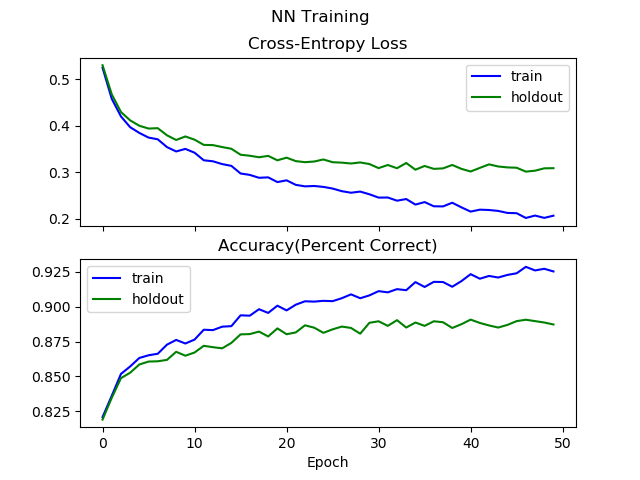
\includegraphics[scale=0.5]{./plots/Training.png}
	\caption{$momentum(\gamma) = 0.9$ , Cross-Entropy Loss \& Accuracy vs epoch}
\end{figure}




\section{Experiment with Regularization}
We test different L2 penalty regularizors in this section. i.e. we choose different $\lambda$ values in the regularizor term $\lambda (\parallel w \parallel_2^2+\parallel b \parallel_2^2)$ of loss function. \\
Figure 2 shows the result, and with $\lambda = 0.001$, we get a final test accuracy of 0.8728. \\
Figure 3 shows the result, and with  $\lambda = 0.0001$, we get a final test accuracy of 0.873. \\
\begin{figure}[h]	
	\centering
	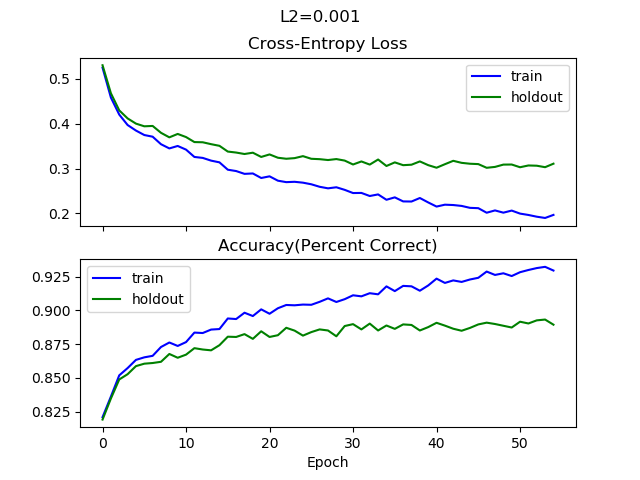
\includegraphics[scale=0.5]{./plots/001Regular.png}
	\caption{$\lambda = 0.001$ , Cross-Entropy Loss \& Accuracy vs epoch}
\end{figure}
\begin{figure}[h]	
	\centering
	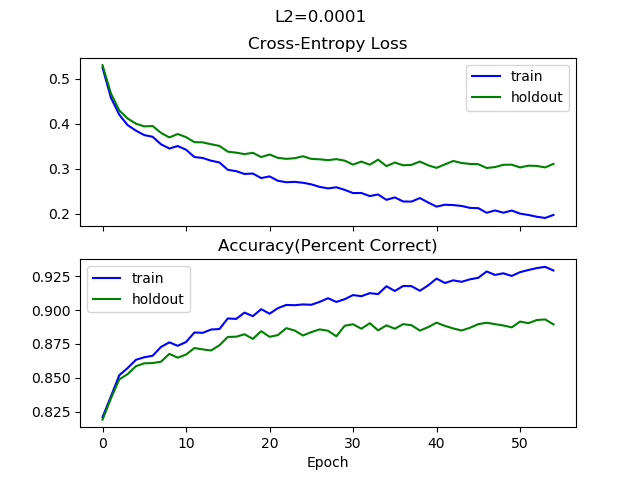
\includegraphics[scale=0.5]{./plots/0001Regular.png}
	\caption{$\lambda = 0.0001$ , Cross-Entropy Loss \& Accuracy vs epoch}
\end{figure}
The performance is almost the same compared with no regularization, maybe because the task is quite easy here. 

\section{Experiment with Activations}
In this section, we experiment with different activation functions.Figures below show the loss and accuracy during training process.\\
Figure 4 uses $tanh$ as our activation, and the final test accuracy is 0.8758. \\
Figure 5 uses  $sigmoid$ as our activation, and the final test accuracy is 0.8684. \\
Figure 6 uses  $ReLU$ as our activation, and the final test accuracy is 0.8762. \\
\begin{figure}[h]	
	\centering
	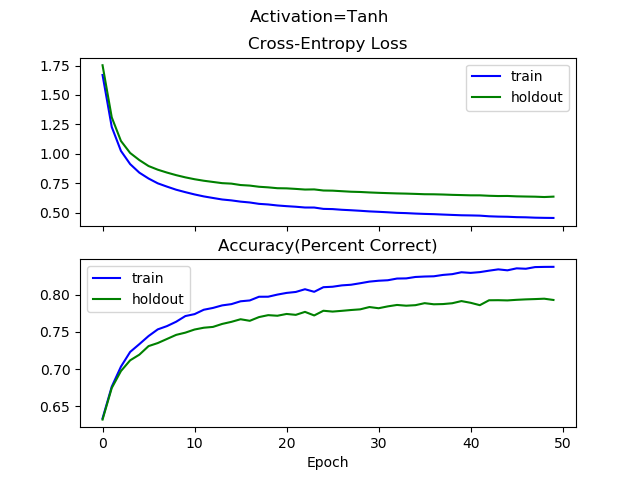
\includegraphics[scale=0.5]{./plots/TanhActivation.png}
	\caption{activation = $tanh$ , Cross-Entropy Loss \& Accuracy vs epoch}
\end{figure}
\begin{figure}[h]	
	\centering
	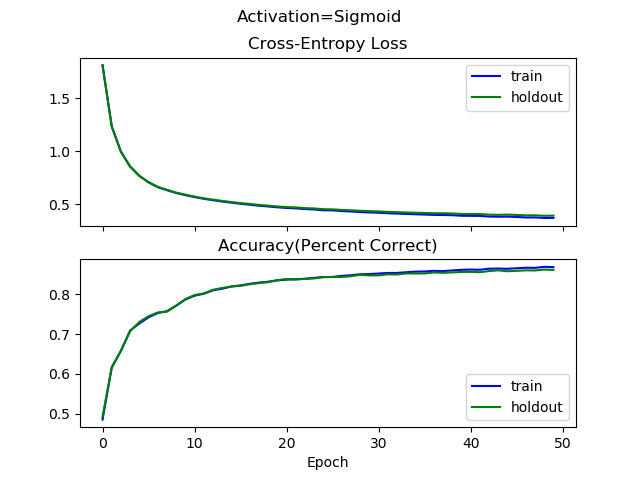
\includegraphics[scale=0.5]{./plots/SigmoidActivation.png}
	\caption{activation = $sigmoid$, Cross-Entropy Loss \& Accuracy vs epoch}
\end{figure}
\begin{figure}[h]	
	\centering
	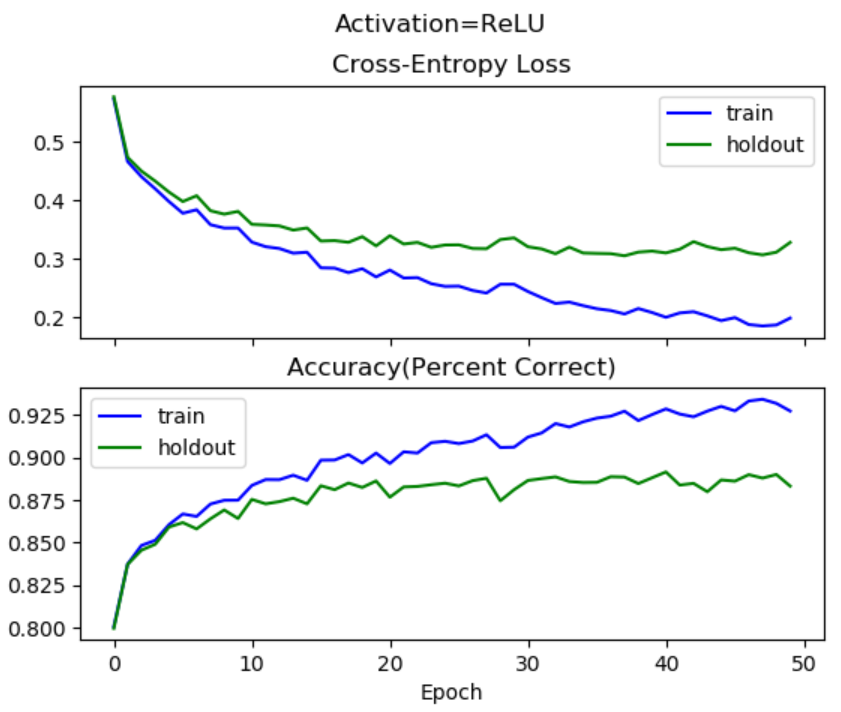
\includegraphics[scale=0.5]{./plots/ReLUActivation.png}
	\caption{activation = $ReLU$ , Cross-Entropy Loss \& Accuracy vs epoch}
\end{figure}
Based on accuracy, $tanh$ and $relu$ both have best performance, but the curve plotted by $sigmoid$ function is smoother than other activation functions. In this problem, $tanh$ is the best activation function.\\

\section{Experiment with Network Topology}
In this section, we experiment with different neural network topology. Figures below show the loss and accuracy during training process. \\
By halving the number of hidden units in Figure 7,i.e. set it to 25, the final test accuracy is 0.8668.\\
By doubling the number of hidden units in Figure 8,i.e. set it to 100, the final test accuracy is 0.8763.\\
We also experiment a neural network with two hidden layers while keeping the same number of total parameters as one 50-unit hidden layer in Figure 9, i.e. two 47-unit hidden layers. The final test accuracy is 0.8766. \\

Here we see that halving the hidden unit number slightly decreases performance and doubling the hidden unit number increases performance. This makes sense because more hidden units allows the neural network to capture more useful features and hence perform better. \\
On the other hand, by extending the neural network's depth while keeping the same number of parameters, the performance increases. Hence we can conclude that depth is important in neural networks.
\begin{figure}[h]	
	\centering
	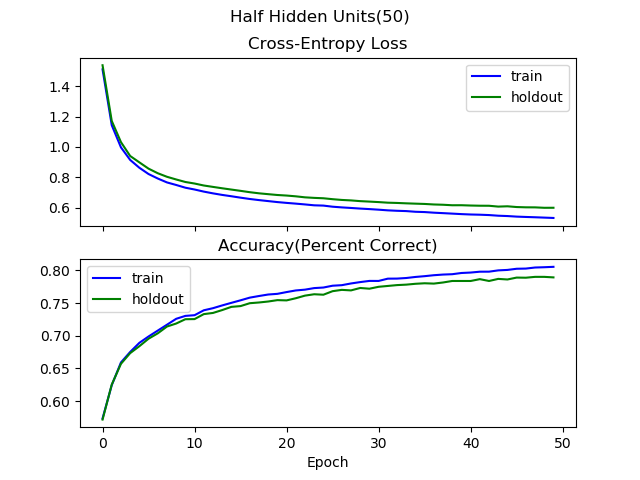
\includegraphics[scale=0.5]{./plots/HalfHiddenUnits.png}
	\caption{Half hidden units , Cross-Entropy Loss \& Accuracy vs epoch}
\end{figure}
\begin{figure}[h]	
	\centering
	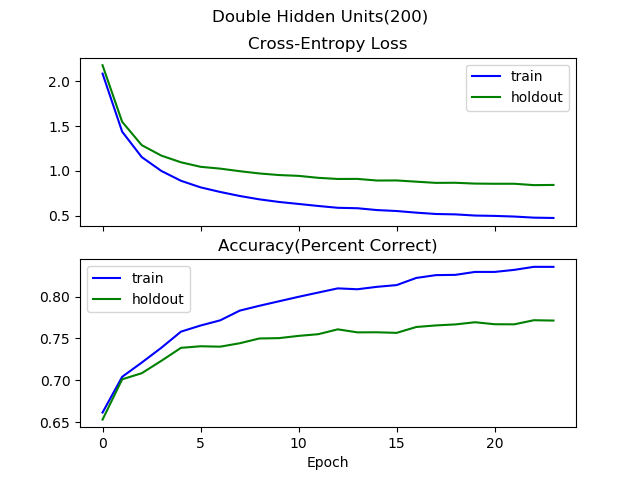
\includegraphics[scale=0.5]{./plots/DoubleHiddenUnits.png}
	\caption{Double hidden units , Cross-Entropy Loss \& Accuracy vs epoch}
\end{figure}
\begin{figure}[h]	
	\centering
	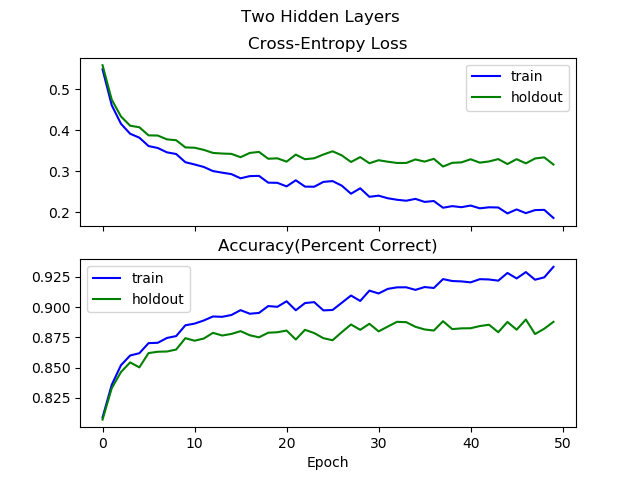
\includegraphics[scale=0.5]{./plots/TwoHiddenLayers.png}
	\caption{Two hidden layers , Cross-Entropy Loss \& Accuracy vs epoch}
\end{figure}
\section{Individual contribution}
Our group consists of two members: \textit{Kexiang Feng} and \textit{Xupeng Yu}. \\
\textit{Kexiang Feng} built the gradient check, and the forward and backward funciton of different activation functions. He also wrote the plotting function.\\
\textit{Xupeng Yu} built the momentum and regularization part. He also finished the main report.
\end{document}